\documentclass{article}
\usepackage{graphicx}
\usepackage{float}

% Margins can be modified here if need be:
\usepackage[a4paper, portrait, left=1cm, right=1cm, top=3cm, bottom=3cm]{geometry}

% Calendar year (for title label) is part of python output:
\newcommand{\CalendarYear}{2022}

\usepackage{array}
% Defining the column format to nicely fill page width:
\newcolumntype{C}{>{\centering\arraybackslash}p{0.12\textwidth}}
% 0.12 is a number I find makes the seven columns fit cleanly in the textwidth with even if margins need to change.

% Document info:
\title{Printable calendar that can be updated by year}
\author{Rachel Ostic}
\date{January 2021}

\begin{document}

% I prefer not to show the page numbers:
\pagenumbering{gobble}
 
% Title page:
\begin{center}
 \section*{\CalendarYear % The title I want on the calendar cover page following the year:
PAINTED MOTH \& BUTTERFLY CALENDAR} 
\end{center}
 
 \begin{figure}[H]
    \centering
    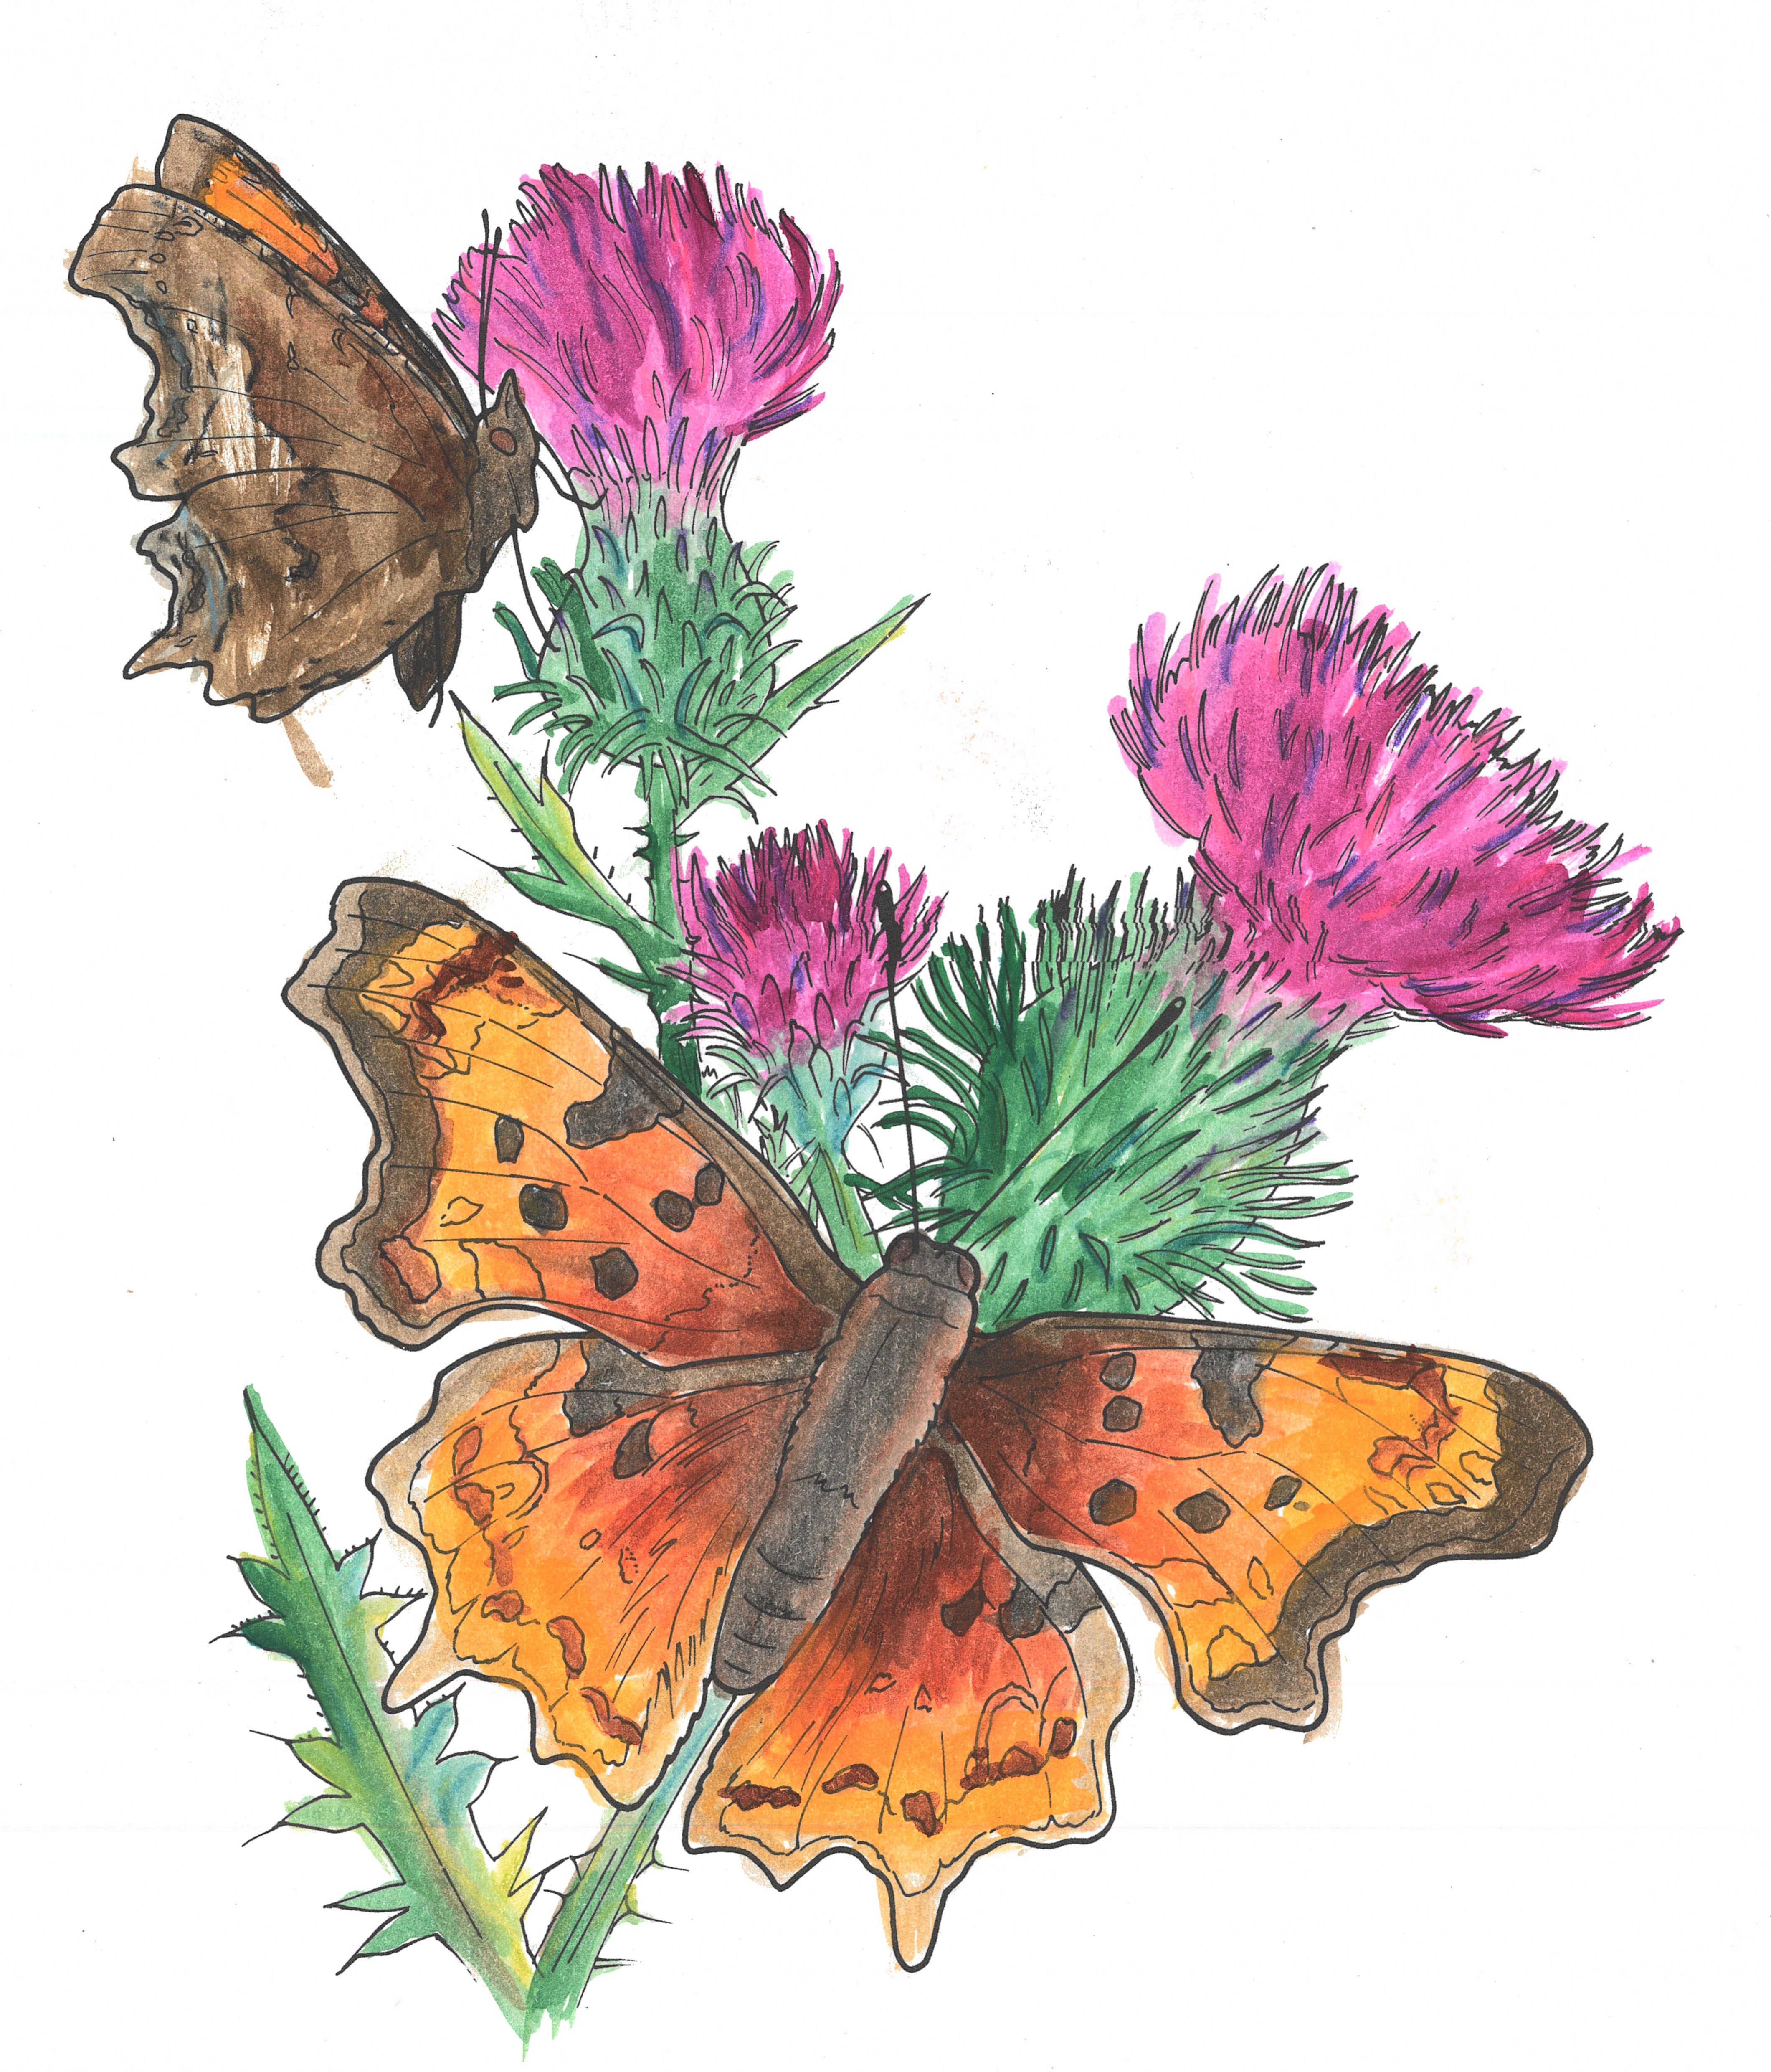
\includegraphics[width=0.95\linewidth]{images/cover.jpg}
\end{figure}
With watercolour illustrations by Rachel Ostic from Ruth Soffer's \textit{Exotic Butterflies and Moths} (Dover, 2002)

% Loop over the months:
\makeatletter

\@for\month:={January,February,March,April,May,June,July,August,September,October,November,December}\do{
\newpage

% month image
 \begin{figure}[H]
    \centering
    \includegraphics[width=\linewidth]{images/\month.jpg}
\end{figure}
\newpage

% month label (not numbered by default, remove * for numbers)
\section*{\month}

% month table
\begin{table}[H]
    \centering
    \begin{tabular}{|*{7}{C|}}
    \hline
    \input{tables/\month.tex} % tex month table generated with python
    \end{tabular}
    \end{table}
    
% monthly caption for image (room for a couple lines - if more space is needed the margins can be decreased, or the calendar cell height can shrink in python table generator)
\input{image-captions/\month-caption}
\newpage
} 

\makeatother



% https://riptutorial.com/latex/example/28657/loops---repeating-things
% used to figure out how to make the loop!!

\end{document}
